% Metódy inžinierskej práce
\documentclass[8pt,oneside,slovak,a4paper]{article}
\usepackage[slovak]{babel}
%\usepackage[T1]{fontenc}
\usepackage[IL2]{fontenc} % lepšia sadzba písmena Ľ než v T1
\usepackage[utf8]{inputenc}
\usepackage{graphicx}
\usepackage{titlesec}
\usepackage{url} % príkaz \url na formátovanie URL
\usepackage{hyperref} % odkazy v texte budú aktívne (pri niektorých triedach dokumentov spôsobuje posun textu)
\usepackage{cite}
%\usepackage{times}
\titlespacing{\section}
{0pt}{0ex}{3ex}
\titlespacing{\subsection}
{0pt}{2ex}{2ex}
\title{Metódy strojového učenia a ich praktické použitie\thanks{Semestrálny projekt v predmete Metódy inžinierskej práce, ak. rok 2021/22, vedenie: Ing. Fedor Lehocki}} 
\author{Martin Orlej\\[2pt]
	{\small Slovenská technická univerzita v Bratislave}\\
	{\small Fakulta informatiky a informačných technológií}\\
	}

\date{\small 6. november 2021} 
\begin{document}
\maketitle
\newpage
\begin{abstract}
Strojové učenie sa v posledných rokoch čoraz viac spomína či už vo vedeckých prácach, alebo v rôznych článkoch, zameraných na technológie. Či už ide o niečo jednoduché, ako aplikácie na telefóny, alebo o vysoko pokročilé technológie ako autonómne jazdenie a počítačové videnie.
\newline \hspace*{0.4cm} V mojej práci by som sa chcel zamerať na rôzne modely strojového učenia, ako napr. lineárna regresia, Naive Bayes a neurónové siete, na ich praktické a najefektívnejšie využitie, napríklad pri spracovávaní veľkého množstva údajov a na slabé miesta a nevýhody týchto modelov.
\newline \hspace*{0.4cm} Rád by som taktiež jednoducho opísal aj už existujúci systém, ako algoritmus GPT-3 vyvinutý nadáciou OpenAI, a možnosti jeho využitia.
\end{abstract}
\section{Úvod} \label {uvod}
Strojové učenie je typ umelej inteligencie, pri ktorom softvér predpovedá výsledok nejakej operácie presnejšie. Strojové učenie sa zameriava na aplikácie a systémy, ktoré sa učia z veľkého množstva údajov a vylepšujú vďaka nim po nejakom čase svoju presnosť, namiesto toho aby boli natvrdo naprogramované. Je veľmi nápomocný hlavne pri praktických úlohách, pri ktorých sa može učiť zo získaných údajov. Čím viac údajov sa do systému strojového učenia vloží, tým viac je daný systém presnejší. 
\newline \hspace*{0.4cm}Strojové učenie je aplikované  v dnešnej dobe takmer všade. Typickým príkladom môže byť predpoveď počasia alebo analýza medicínskych snímok pri diagnostike rakoviny. Používa sa taktiež v robotike, virtuálnych asistentoch (Google, Siri, Alexa), hrách, spracovávaní jazyka a textu, odporúčania produktov v online obchodoch, analýza nákupov zákazníka, vyhľadávačoch (Google Search), detekcia podvodov, boti (Chatbot), filtrovanie spamu a taktiež aj v socíalnych sieťach. 
\newline \hspace*{0.4cm}Existujú dve hlavné metódy strojového učenia, a to Supervised Learning (priradzuje vstupný údaj k výstupu a kontroluje či je výstup modelu správny) a Unsupervised Learning (stroj kontroluje výstupy sám). Každý z týchto systémov má svoje výhody a aj nevýhody.
\subsection{Motivácia} \label{motivacia}
\newpage
\section{Regresia} 
\subsection{Lineárna regresia}
Lineárna regresia je prístup typu Supervised Learning, čiže stroj kontroluje svoje výstupy oproti už daným výstupným údajom. Medzi jej výhody patrí jej jednoduchosť na pochopenie a taktiež schopnosť následne vylepšovať pomocou nových údajov. Tento model je skvelou voľbou pre každého, kto chce začať s dátovou analýzou a strojovým učením. \cite{quick_review}
\newline \hspace*{0.4cm} Ide o jednu z najviac používaných metód strojového učenia. Lineárnu regresiu môžme rozdeliť na tri typy, a to jednoduchú, viacnásobnú a polynomiálnu
\subsection{Decision tree}
Ide o v celku populárny model strojového učenia, ktorý sa používa pri strategickom plánovaní a strojovom učení. Každý štvorec z obrázku sa nazýva uzol, a čím viac uzlov sa v danom strome nachádza, tým viac je tento model presnejší.  Na konci každého uzla sa nachádza tzv. list, ktorý obsahuje tzv. rozhodnutie, teda výstupnú hodnotu podľa podmienok v danom liste, do ktorého sa systém dostal. 
\newline \hspace*{0.4cm} Medzi výhody tohto modelu patrí jeho možnosť využitia pri regresii a klasifikácií, jednoduchosť pri spracúvavaní kategorických a kvantitatívnych hodnôt a aj prípadnom dopĺňaní chýbajúcich hodnôt s najviac pravdepodobnou hodnôtou.
V praxi je jednoduché vybudovať decision tree model, no jeho nedostatkom je jeho presnosť. \cite{quick_review}
\begin{figure}[h]
\centering
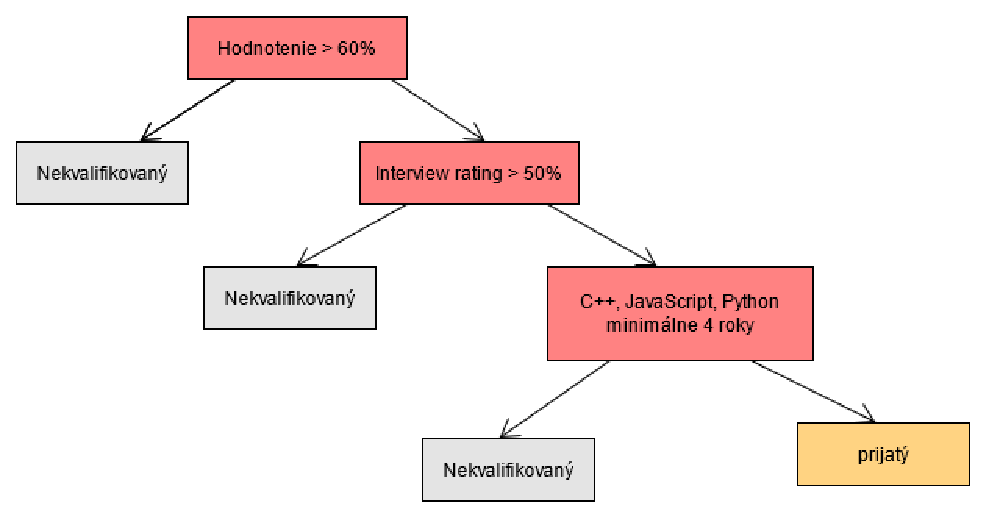
\includegraphics[scale=0.55]{decision_tree}
\caption{Príklad Decision Tree modela}
\end{figure}
\newpage
\section{Klasifikácia}
\subsection{Logická regresia}
Logická regresia funguje podobne ako lineárna regresia, ale používa sa na modelovanie určitého množstva výsledkov, zvyčajne dvoch. V jednoduchosti, logická rovnica používaná pri tomto modeli je vytvorená tak, že výstupná hodnota je vždy medzi hodnotami 0 a 1;
\subsection{Naive Bayes}
Naive Bayes je jedným z populárnych klasifikátorov používaným v strojovom učení. Hlavnou ideou za týmto modelom je Bayesova veta.
\begin{equation} \label{bayes_eq}
 \Pr(A|B)=\frac{\Pr(B|A)\Pr(A)}{\Pr(B)}
\end{equation}
\begin{figure}[h]
\centering
\ref{bayes_eq}Vzorec č.1  Bayesova veta \cite{bayes_equation}
\end{figure}
\newline Výhody tohto modelu sú jednoduchá implementácia, skvelý výkon, dokáže pracovať s nižším objemom údajov, dokáže pracovať s binárnou a viactriednou klasifikáciou a vytvárať pravdepodobnostné predpovede. \newline \hspace*{0.4cm} Modely strojového učenia, ktoré sú riadne natrénované a optimalizované väčšinou prekonajú modely typu Naive Bayes. \cite{quick_review}
\subsection{Neurónová sieť} 
Neurónová sieť je v jednoduchom pojímaní len sieť matematických rovníc. Delí sa na tri základné časti, a to vstupná vrstva, ktorá prijíma údaje, potom následuje skrytá vrstva a na záver výstupná vrstva. Každý uzol v skrytej vrstve predstavuje zároveň lineárnu funkciu a tzv. aktivačnú funkciu.
\begin{figure}[h] 
\centering
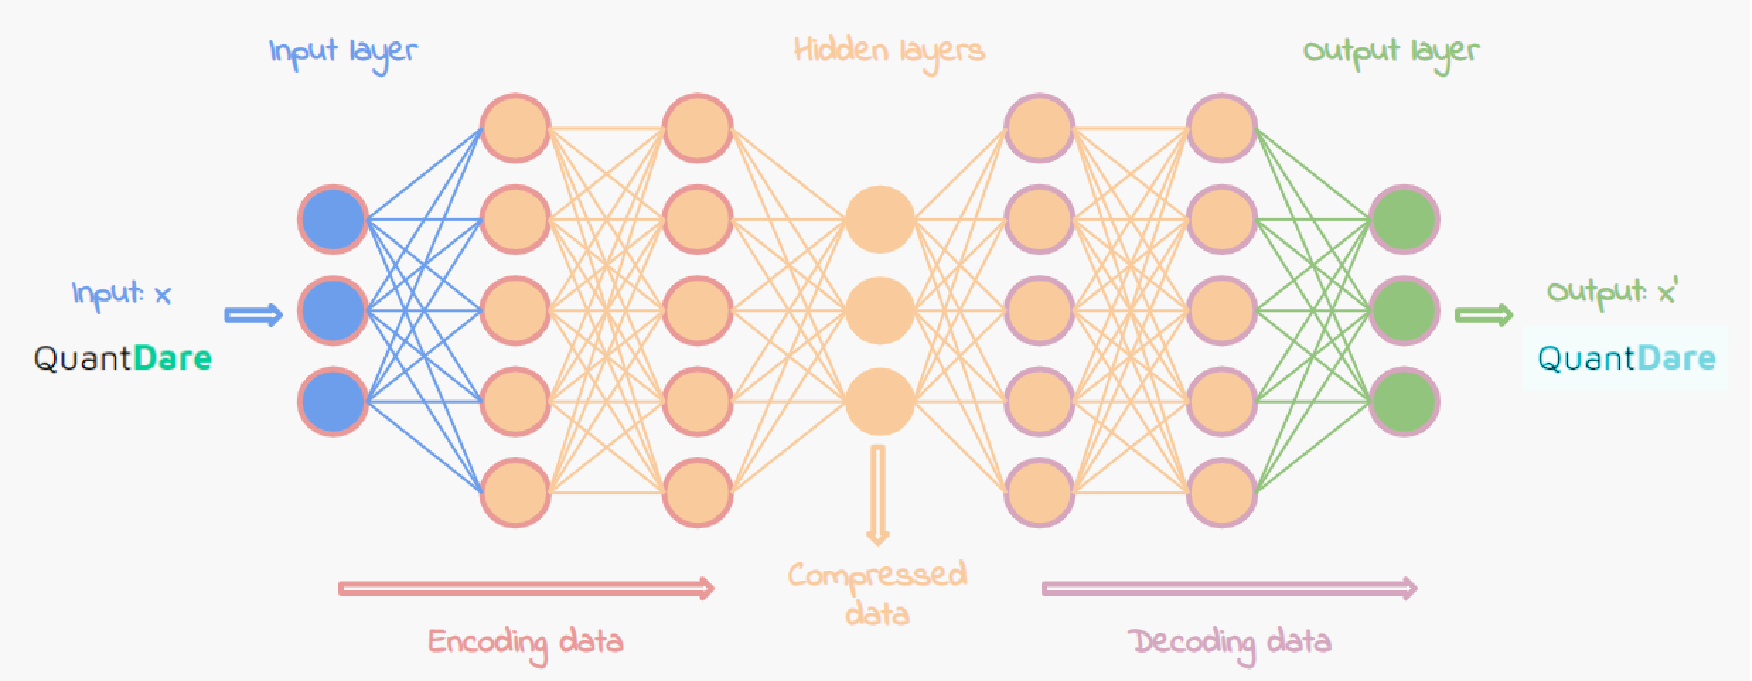
\includegraphics[scale=0.4]{neural_network_img}
\caption{Zjednodušený model neurónovej siete \cite{neural_network_image}}
\end{figure}
\newpage
\section{Praktické využitie strojového učenia} \label{vyuzitie}
\subsection{Každodenné použitie}
\subsection{Medicína}
K jedným z praktických využití v medicíne patrí aj analýza medicínskych údajov a snímok o pacientovi a ich následne vyhodnocovanie. \cite{heart_disease}
\subsection{Spracovávanie dát}
\subsection{Model GPT-3}
Model GPT-3 bol vytvorený výskumnym laboratóriom OpenAI, ktorého cieľom je vytvoriť priateľskú umelú inteligenciu, ktorá by ľudom pomáhala.\cite{GPT3} Ide o model hlbokého učenia, ktorý sa prevažne používa pri spracovávaní  prirodzeného jazyka a počítačovom videní. Transformátory pracujú s určitou sekvenciou dát, ktorá sa ale nemusí spracovávať zaradom, ako pri iných modeloch.\newline \hspace*{0.4cm} Systém GPT-3, ako už jeho názov naznačuje, je v poradí treťou generáciou tohto modelu v podaní OpenAI. Jeho cieľom je vytvárať text, ktorý je bežným ľudským okom prakticky nerozoznateľný od textu ktorý by napísal človek. A tento text sa generuje len z nejakého jednoduchého vstupu, ktorý používateľ zadá. Pri trénovaní podobných algoritmov sa bežne používa obrovská databáza slov, v tomto prípade išlo o 175 miliard slov.\cite{GPT3}

\newpage
\section{Záver} \label{zaver}
\subsection{Diskusia} \label{diskusia}

\bibliography{literatura}
\bibliographystyle{plain} 
\end{document}